%Autores: Felipe
%         Igor
%       Lucas
%       Thalis
%Contato: phyllipe_slf@yahoo.com.br
%         biblioteca.pesquisa@inatel.br
%Modelo para escrita de artigos científicos para o TCC dos cursos Graduação do INATEL - Instituto Nacional de Telecomunicações. 
%Este template LaTeX é uma adaptação do modelo doc desenvolvido pelos professores Carlos Ynoguti e Dayan Guimarães

%Se você é novo no latex, um bom lugar para começar é
%https://pt.overleaf.com/learn
\documentclass[10pt,twocolumn]{article} 
%Use esse arquivo para incluir novos pacotes

\usepackage[%usado para determinar medidas
top=1.78cm,
bottom=1.78cm,
left=1.65cm,
right=1.65cm,
headsep=0cm,
%showframe
]{geometry}
%\usepackage[justification=centering]{caption}
\usepackage{inatel}%carregar algumas estilizacoes do inatel
\usepackage{times}
\usepackage{enumitem}%redefinir espacos itemize
\usepackage{graphicx}
\usepackage[hyphens]{url}
\usepackage{hyperref}
\usepackage[utf8]{inputenc}
\usepackage{float}%mais controle para manipular figuras
\usepackage{caption}%manipular legenda da figura e tabela
\usepackage{mathtools}%equacoes
\usepackage[hang,flushmargin]{footmisc} 
\usepackage{xcolor}
\usepackage{wrapfig} %usado para envolver figura com texto
%\usepackage[portuguese]{babel}
\usepackage{fancyhdr}%criacao do cabecalho
\usepackage{etoolbox}
\usepackage{adjustbox}%mais controle para ajustar tamanho da tabela
\usepackage{comment}%ambiente para comentario
\usepackage{relsize} %usado por comandos \mathlarger
%\usepackage{mathptmx}
\usepackage{csquotes}

%Referencia bibliografica
\usepackage[
    style=numeric,
    sorting=none,
    maxbibnames=10]{biblatex}
\addbibresource{referencia.bib}

%Idioma. Use "english" para trabalhos em inglês
\usepackage[brazil]{babel}

%Ajustes na legenda da figura. Incluindo espacamento apos a legenda
\captionsetup[figure]{labelformat={default},labelsep=period,font=footnotesize, name=\footnotesize{Fig.},justification=raggedright,singlelinecheck=false,belowskip=-0.9\normalbaselineskip}
%\pagenumbering{gobble}

%Ajustes na legenda da tabela. 
%\captionsetup[table]{labelformat={default},labelsep=newline,font={sc,footnotesize},name=\footnotesize{TABELA}}

\renewcommand{\headrulewidth}{0pt}


\begin{document}

\title{\Huge \bf Price Search: um projeto de código aberto para busca e comparação de preços em estabelecimentos locais}

\author{
    \begin{tabular}{ccccc}
    Felipe de Cássio Rocha Santos & Igor Galvão de Melo & Lucas Jose Silva Correa & Thalis Andrade Oliveira de Souza & Marcelo Vinícius Cysneiros Aragão \\
    \multicolumn{5}{c}{Instituto Nacional de Telecomunicações - Inatel} \\
    \multicolumn{5}{c}{\{felipe.santos,igorgalvao,lucas.jose,thalisandrade,marcelovca90\}@gec.inatel.br}
    \end{tabular}
}

\maketitle

\noindent\blfootnote{Trabalho de Conclusão de Curso apresentado ao Instituto Nacional de Telecomunicações, como parte dos requisitos para a obtenção do Grau de Bacharel em (nome do curso). Orientador: Prof. (XXXXX). Trabalho aprovado em XX/20XX.}

\begin{abstract}
This document is about the development of a web application, for price comparison in local establishments, using the product search and a database. It explains how other projects interacted with the end user, in order to provide the result of researching the price of a product online; and the technologies that support the completion of the final project.
\end{abstract}

\begin{keywords}
Mobile application, comparison, purchase, online, price, product.
\end{keywords}

\begin{resumo}
Este documento é sobre o desenvolvimento de um aplicativo web, para comparação de preço em estabelecimentos locais, usando a pesquisa de produtos e um banco de dados. Nele é explicado a forma com que outros projetos interagiam com o usuário final, a fim de fornecer o resultado da pesquisa do preço de um produto online; e as tecnologias que favorecem a conclusão do projeto final.
\end{resumo}

\begin{palavrasChaves}
Aplicação web, comparação, compra, online, preço, produto.
\end{palavrasChaves}


\section{Introdução}

O propósito deste documento é fornecer informações para ajudar os autores a produzir artigos com aparência profissional para a Revista Telecomunicações. Esse modelo LaTeX foi adaptado do modelo doc feito pelos Professores Carlos Alberto Ynoguti e Dayan Adionel Guimarães.


\section{Ferramentas}

\subsection{Angular}
Angular \cite{afonso2018angular} é uma plataforma e \textit{framework} para construção da interface de aplicações usando HTML (do inglês, \textit{HyperText Markup Language}), CSS (do inglês, \textit{Cascading Style Sheets}) e, principalmente, JavaScript, criada pelos desenvolvedores da Google. 

Ele possui basicamente dois tipos: AngularJs e o Angular 2+; que são tecnologias completamente diferentes. O AngularJs é um framework baseado totalmente em JavaScript para desenvolvimento web e o Angular 2+ que surgiu para desenvolvimento não só web, mas também para mobile, usa o TypeScript, e que teve várias mudanças no modo de construção da aplicação.A arquitetura do Angular permite organizar a aplicação por módulos através dos NgModules\footnote{Lorem ipsum dolor sit amet.}, que fornecem um contexto para os componentes serem compilados. 

Uma aplicação sempre tem ao menos um módulo raiz que habilita a inicialização e, normalmente, possui outros módulos de bibliotecas. Os componentes deliberam as visualizações — que são conglomerados de elementos e funcionalidades de tela — que o Angular modifica de acordo com a lógica e os dados da aplicação[2].O Angular também possui uma ferramenta chamada Angular CLI, que permite criação de utensílios que auxiliam que são necessário, como: componentes, serviços, interfaces, etc. Segue abaixo algumas vantagens do uso do Angular:  

\begin{itemize}
    \item Produtividade: desenvolver uma aplicação com ele requer bem menos código, sendo inclusive intuitivo e dando suporte para a modularização; 
    \item Fácil manuseamento: muito fácil entender o funcionamento das aplicações lendo apenas o HTML;   
    \item Criação de frameworks: é possível criar nosso próprio framework a partir dele;   
    \item Teste unitário: é simples, pois toda a estrutura é desacoplada e as dependências são injetadas, o que facilita a criação de fakes, stubs, spies e mocks, melhorando – e muito – todo o processo de teste de controladores, serviços e diretivas. 
\end{itemize}

\subsection{TypeScript}
Tendo escolhido o Angular para trabalhar com o frontend, não teria como utilizar do mesmo para desenvolver o backend, já que o Angular não é uma boa linguagem e nem possui características para isso. Portanto, para a parte de backend escolhemos o TypeScript, que é uma linguagem de programação \textit{open-sorce} desenvolvido pela \textit{Microsoft} 

\subsection{NestJS}
O NestJS cria uma camada de abstração em cima de uma das bibliotecas mais utilizadas para criação de aplicações web no mundo, o Nodejs.  Então é muito difícil comentar sobre um, sem mencionar o outro, é preciso ressaltar que deve-se ter instalado em sua máquina o Nodejs para que seja possível utilizar do Nestjs. O Nestjs é uma estrutura para criar aplicativos de forma eficiente, ele conta com um CLI (Command Line Interface) que permite a criação e configuração inicial do projeto.

O Nestjs fornece uma arquitetura de aplicativos pronta para uso que permite que desenvolvedores e equipes criem aplicativos altamente testáveis, escaláveis, com acoplamentos frouxos e de fácil manutenção \cite{kamil2020nestjs}. Segue abaixo algumas vantagens do NestJS .

\begin{itemize}
    \item A estrutura de pastas no Nest é fortemente baseada em Angular; 
    \item A estrutura é muito orientada a anotações, e as anotações tornam o desenvolvimento mais simples;   
    \item Ferramenta de linha de comando permitirá monitorar o projeto, gerar componentes da arquitetura Nest e exibir informações do projeto;   
\end{itemize}

\subsection{Visual Studio Code}
Como IDE (\textit{Integrated Development Environment}) a ferramenta escolhida para ser utilizada foi o Visual Studio Code que é um editor de código-fonte desenvolvido pela Microsoft para Windows, Linux e macOS. A escolha dessa ferramenta foi devido ser \textit{open source}, possuir suporte para o Git e a abrangência que ela traz para aplicação de \textit{plugins}, ou seja, mecanismos que facilitam na programação para a devida linguagem escolhida.

Com suporte para centenas de idiomas, o VS Code ajuda você a ser instantaneamente produtivo com realce de sintaxe, correspondência de colchetes, recuo automático, seleção de caixa, trechos e muito mais. Atalhos de teclado intuitivos, personalização fácil e mapeamentos de atalhos de teclado contribuídos pela comunidade permitem navegar com facilidade pelo seu código. \cite{mjbvz2020VSCode}


\subsection{Gitpod}
Como o GitHub possui recursos limitados para edição, forçando muitas vezes os usuários utilizar de recursos locais em suas máquinas para resolver até pequenos problemas, o Gitpod surge como uma luz para os amantes de GitHub. Ele não é simplesmente uma IDE online, ele é muito mais do que isso, ele é como uma extensão para edição do GitHub, usando como IDE base o Visual Studio Code. 

Diferentemente dos IDEs tradicionais da nuvem e da área de trabalho, o Gitpod entende o contexto e prepara o IDE automaticamente. Por exemplo, se você estiver criando um espaço de trabalho Gitpod a partir de uma solicitação pull do GitHub, o IDE será aberto no modo de revisão de código. Além disso, os espaços de trabalho do Gitpod devem ser descartáveis. Ou seja, você não precisa manter nada. Eles são criados quando você precisar deles, e você pode esquecê-los quando terminar \cite{jankeromnes2020Gitpod}. 


\subsection{Swagger}
A ferramenta Swagger é outra que não poderia faltar no projeto, feita para modelagem, documentação e geração de código para APIs do estilo REST, seja manualmente ou geradas automaticamente a partir do código-fonte, traz uma enorme vantagem para quem deseja trabalhar com testes de APIs. A capacidade das APIs de descrever sua própria estrutura é a raiz de toda a grandiosidade do Swagger.

Podemos criar automaticamente uma documentação API bonita e interativa. Também podemos gerar automaticamente bibliotecas de clientes para sua API em vários idiomas e explorar outras possibilidades, como testes automatizados. O Swagger faz isso solicitando que sua API retorne um YAML ou JSON que contenha uma descrição detalhada de toda a API. Este arquivo é essencialmente uma lista de recursos da sua API que adere à especificação \textit{OpenAPI} \cite{shockey2020Swagger}. A especificação solicita que você inclua informações como:

\begin{itemize}
    \item Quais são todas as operações suportadas pela sua API? 
    \item Quais são os parâmetros da sua API e o que ela retorna?   
    \item Sua API precisa de alguma autorização?
    \item E até coisas divertidas, como termos, informações de contato e licença para usar a API.
\end{itemize}

\

\section{Instruções Gerais}
Quando escrever o seu artigo, por favor atente às seguintes instruções:

\subsection{Tamanho e formato do papel}
Os trabalhos serão impressos em papel tamanho carta (letter), exatamente como você os submeter. Desta forma, a organização e o esmero são de extrema importância. Por favor, faça uma revisão cuidadosa dos erros gramaticais e de digitação antes da submissão. Não há limite de páginas, e contamos com o bom senso dos autores neste caso. Os artigos devem ser preparados em coluna dupla. Defina as margens superior e inferior em 1,78 cm, as margens esquerda e direita em 1,65 cm. As colunas devem ter largura de 8,89 cm e o espaço entre elas devem ser de 0,51 cm. Use espaçamento simples entre as linhas.

\subsection{Resumo e abstract}
Os artigos escritos em língua portuguesa devem ter também o resumo e as palavras-chave traduzidos para a língua inglesa, como neste exemplo. Garanta que tanto o abstract quanto o resumo tenham no máximo 150 palavras.

\subsection{Seções e subseções}
As seções devem ser numeradas com algarismos romanos e ter o título centralizado. Já as subseções devem ser numeradas com letras maiúsculas e ter o título justificado, caso haja sequência de subtítulos as letras devem ser minúsculas e justificadas. 

\subsubsection{Sub-subseções}
Este é um exemplo de sub-subseção, mas ela deve ser evitada na escrita de artigo científico. A necessidade de usar sub-subseções pode indicar um problema de estruturação do artigo.

\subsection{Figuras e Tabelas}
Figuras e Tabelas devem ser incluídas como parte do texto sempre que possível; caso contrário, agrupe-as ao final do texto. As Figuras não devem ter elementos coloridos e seus títulos devem ser posicionados depois das mesmas, com alinhamento justificado. A sua numeração deve ser feita com algarismos arábicos. Para as Tabelas, o procedimento é diferente: seus títulos devem ser posicionados antes das mesmas, centralizados, e a numeração deve ser feita com algarismos romanos. Na Figura \ref{fig:revista_inatel} tem-se um exemplo de uma figura:

\begin{figure}[H]
  \centering
  
\includegraphics[width=0.22\textwidth]{figuras/figura1.png}
  \caption{Uma figura. O título deve ser colocado abaixo da mesma.}
  \label{fig:revista_inatel}
\end{figure}

\subsection{Equações}
A numeração das equações deve ser entre parênteses e alinhada à direita, como no exemplo abaixo:

\begin{equation}
\mathbf{\mathit{\mathlarger{\phi}_{X}(s) = E[\mathrm{e}^{sx}]}}
\end{equation}

%Consulte a página 
para mais símbolos matemáticos, consulte o LaTeX wiki%\footnote{\url{https://en.wikibooks.org/wiki/LaTeX/Mathematics}} 

\subsection{Fontes}

Use fonte do tipo Times New Roman ou similar. Os tamanhos a serem usados são mostrados na Tabela \ref{tab:tabela1}

\begin{table}[h]
\caption{Tamanhos e Tipos de Letras}
\label{tab:tabela1}
\begin{adjustbox}{max width=\textwidth}
\begin{tabular}{|c|c|c|}
\hline
TEXTO & TAMANHO & ESTILO \\ \hline\hline
Título                      & 24pt                         & Negrito                     \\
Nome do autor               & 11pt                         & Normal                      \\
Afiliação                   & 10pt                         & Normal                      \\
Texto principal             & 10pt                         & Normal                      \\
Título das seções           & 10pt                         & Caixa Alta                  \\
Título das subseções        & 10pt                         & Itálico                     \\
Título do resumo/abstract   & 9pt                          & Negrito,Itálico             \\
Resumo/Abstract             & 9pt                          & Negrito                     \\
Título das figuras          & 8pt                          & Normal                      \\
Título das tabelas          & 8pt                          & Caixa Alta                  \\
Texto das tabelas           & 8pt                          & Normal                      \\
Referências                 & 8pt                          & Normal                      \\ \hline
\end{tabular}
\end{adjustbox}
\end{table}


%Se desejar, consulte a página \url{https://www.tablesgenerator.com} para criar a estrutura da sua tabela em latex. Esta página fornece uma interface gráfica que facilita a geração de tabelas em latex. Depois de gerado o código fonte pela página, insira este código no seu texto e faça os ajustes necessários.

\subsection{Referências bibliográficas}

Liste as referências em ordem numérica ao final do artigo. Ao final deste texto tem-se vários exemplos de como listá-las, dependendo do tipo. Denote as citações dentro do texto através de colchetes (por exemplo \cite{LIMA2018}). Ao referenciar mais de um trabalho, use o mesmo par de colchetes, como exemplo: \cite{LIMA2018, schell2014, Lima2017}. 

Segue um exemplo para citações textuais: ``De acordo com \textcite{LIMA2018}'' 


\subsection{Outras questões}
Não use notas de rodapé a menos que sejam estritamente necessárias; neste caso, procure não agrupá-las. 
\section{Conclusão}
A seção de conclusões não é obrigatória. Embora esta possa rever os pontos principais do artigo, não duplique o resumo como conclusão. A conclusão deve discorrer sobre a importância do trabalho ou sugerir aplicações e extensões.

%Exemplo de comentario
\begin{comment}
Aqui também é um comentário
\end{comment}
\section*{Autores}

\begin{wrapfigure}{l}{0.3\linewidth}

\includegraphics[width=\linewidth]{figuras/autor1.png}
\end{wrapfigure}

    \textbf{Phyllipe Lima} é Doutorando em Computação Aplicada pelo INPE - Instituto Nacional de Pesquisas Espaciais, na área de Engenharia de Software realizando estudos sobre metadados através da análise estática de código fonte e MSR (Mining Software Repositories). Mestre em Ciência da Computação(2016) pela UNIFEI - Universidade Federal de Itajubá. Engenheiro de Telecomunicações(2011) pelo INATEL - Instituto Nacional de Telecomunicações.  Técnico em Telecomunicações(2006) pela Escola Técnica de Eletrônica - ETE "FMC". É professor auxiliar do INATEL, atuando nos cursos de Engenharia da Computação e Engenharia de Software. Tem interesse nas áreas de Engenharia de Software Empírica, Desenvolvimento de Jogos e Computação Gráfica\newline

\begin{wrapfigure}{l}{0.3\linewidth}
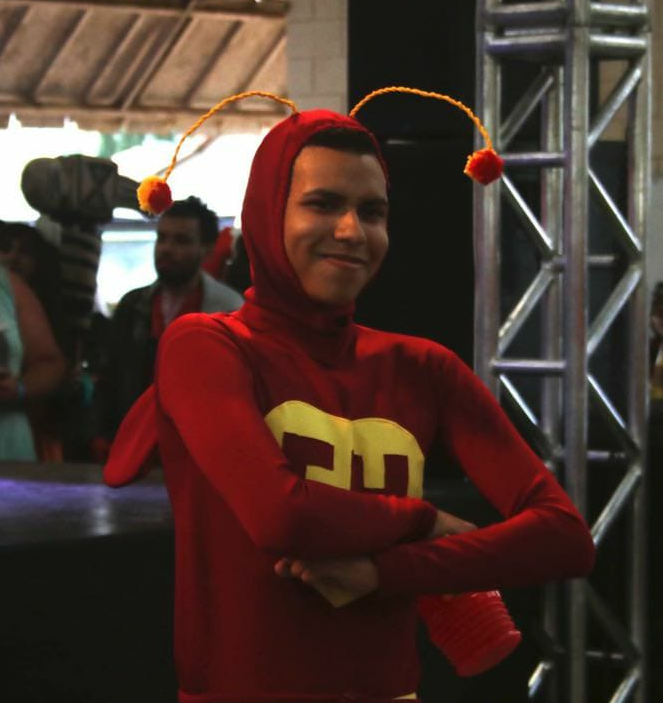
\includegraphics[width=\linewidth]{figuras/autor2.png}  
\end{wrapfigure}

   \textbf{Daylon Ramos} é graduando em Tecnologia em Gestão de Telecomunicações pelo INATEL - Instituto Nacional de Telecomunicações. Bolsista na Biblioteca Ministro Olavo Bilac Pinto - INATEL. Tem interesse nas áreas de Tecnologia, Gestão e Engenharia de Produção.


\printbibliography

\section*{Autores}

\begin{wrapfigure}{l}{0.3\linewidth}

\includegraphics[width=\linewidth]{figuras/autor1.png}
\end{wrapfigure}

    \textbf{Phyllipe Lima} é Doutorando em Computação Aplicada pelo INPE - Instituto Nacional de Pesquisas Espaciais, na área de Engenharia de Software realizando estudos sobre metadados através da análise estática de código fonte e MSR (Mining Software Repositories). Mestre em Ciência da Computação(2016) pela UNIFEI - Universidade Federal de Itajubá. Engenheiro de Telecomunicações(2011) pelo INATEL - Instituto Nacional de Telecomunicações.  Técnico em Telecomunicações(2006) pela Escola Técnica de Eletrônica - ETE "FMC". É professor auxiliar do INATEL, atuando nos cursos de Engenharia da Computação e Engenharia de Software. Tem interesse nas áreas de Engenharia de Software Empírica, Desenvolvimento de Jogos e Computação Gráfica\newline

\begin{wrapfigure}{l}{0.3\linewidth}
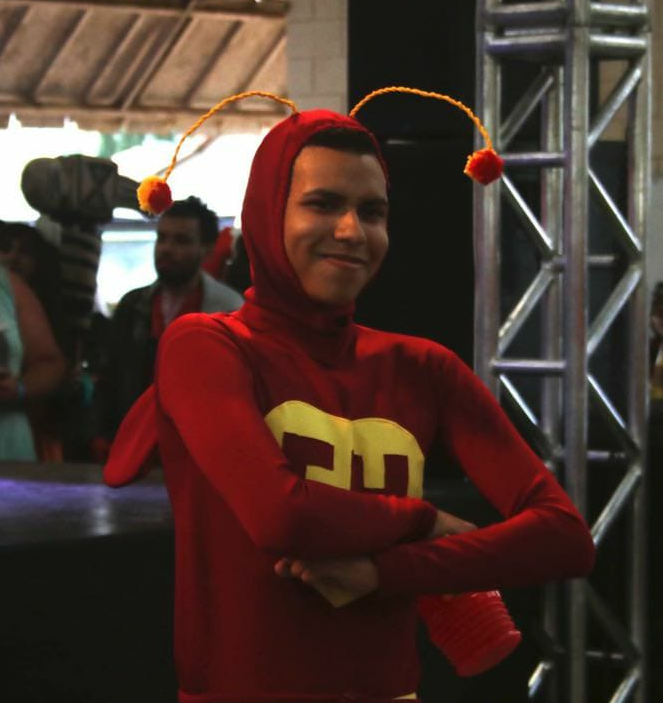
\includegraphics[width=\linewidth]{figuras/autor2.png}  
\end{wrapfigure}

   \textbf{Daylon Ramos} é graduando em Tecnologia em Gestão de Telecomunicações pelo INATEL - Instituto Nacional de Telecomunicações. Bolsista na Biblioteca Ministro Olavo Bilac Pinto - INATEL. Tem interesse nas áreas de Tecnologia, Gestão e Engenharia de Produção.

\end{document}